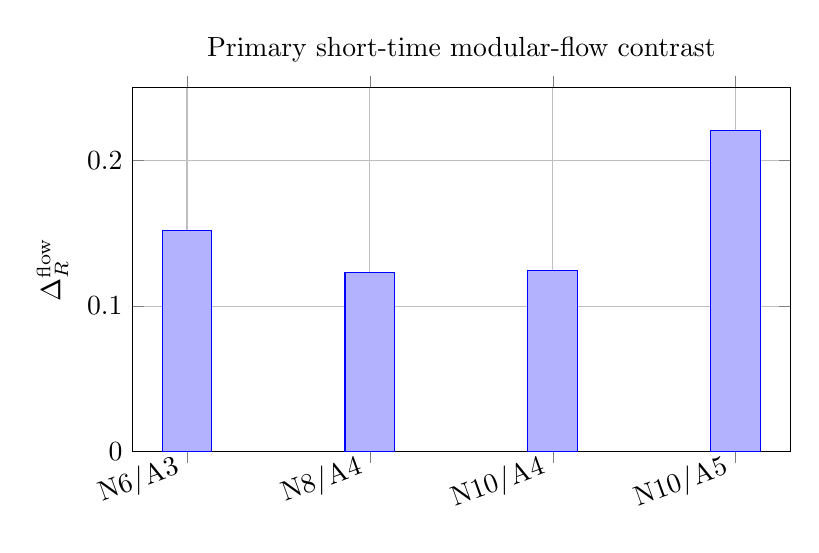
\begin{tikzpicture}
\begin{axis}[
  width=0.82\textwidth,height=6.2cm,
  ybar,bar width=18pt,
  ymin=0,ymax=0.25,
  ylabel={$\Delta_R^{\rm flow}$},
  symbolic x coords={N6/A3,N8/A4,N10/A4,N10/A5},
  xtick=data,
  x tick label style={rotate=20,anchor=east},
  title={Primary short-time modular-flow contrast},
  grid=major
]
\addplot coordinates {(N6/A3,0.1519583896) (N8/A4,0.1229235652) (N10/A4,0.1241991943) (N10/A5,0.2208624919)};
\end{axis}
\end{tikzpicture}
